\documentclass[11pt,spanish,listoffigures]{tfgetsinf}
\usepackage[utf8]{inputenc} 

%%%%%%%%%%%%%%%%%%%%%%%%%%%%%% PORTADA %%%%%%%%%%%%%%%%%%%%%%%%%%%%%%

\title{Implementación y despliegue de un proxy inverso para una arquitectura de microservicios}
\author{Alejandro Carrión Sanmartín}
\tutor{Patricio Letelier Torres}
\curs{2020-2021}

%%%%%%%%%%%%%%%%%%%%%%%%%%%%%% PALABRAS CLAVE %%%%%%%%%%%%%%%%%%%%%%%%%%%%%%

\keywords{????, ?????????} % Paraules clau 
         {?????, ???} % Palabras clave
         {?????, ?????} % Key words

\begin{document}

%%%%%%%%%%%%%%%%%%%%%%%%%%%%%% RESUMEN %%%%%%%%%%%%%%%%%%%%%%%%%%%%%%

\begin{abstract}[spanish]
????
\end{abstract}
\begin{abstract}[catalan]
????
\end{abstract}
\begin{abstract}[english]
????
\end{abstract}

\mainmatter

%%%%%%%%%%%%%%%%%%%%%%%%%%%%%% INTRODUCCIÓN %%%%%%%%%%%%%%%%%%%%%%%%%%%%%%

\chapter{Introducción}

El uso de arquitecturas de microservicios es una práctica ya consolidada hoy en día en el mundo del desarrollo de \emph{software}. Esta consiste en la construcción de servicios independientes, ejecutados en procesos diferentes, que se encargan de realizar funciones concretas y que trabajan de forma conjunta para lograr el objetivo u objetivos globales de la aplicación que constituyen. Los beneficios que otorga este enfoque frente a la aproximación tradicional monolítica son muchos y muy variados. Algunos de ellos son:

\begin{itemize}

	\item \textbf{Uso de diferentes tecnologías}.
Cada microservicio puede estar construido con una tecnología diferente y puede utilizar distintos mecanismos de persistencia.

	\item \textbf{Maniobrabilidad en los despliegues}.
Ante cualquier cambio no es necesario desplegar la aplicación entera, solamente los microservicios implicados.

	\item \textbf{Tolerancia a fallos}.
La posibilidad de desplegar la aplicación de forma que quede repartida en diferentes máquinas, incluso duplicando microservicios, otorga cierta capacidad para tolerar fallos.

	\item \textbf{Escalabilidad y mantenibilidad}.
Los microservicios, y la separación funcional que otorgan, facilitan el escalado de las diferentes partes de la aplicación de manera independiente. Lo mismo sucede con el mantenimiento, pudiendo crear equipos especializados.

\end{itemize}

Se puede obtener más información acerca de los microservicios en el artículo de James Lewis y Martin Fowler titulado ''\emph{Microservices}'' \cite{LewisAndFowler}. Para una lectura con más profundidad, el libro ''\emph{Building Microservices} \cite{Newman}'' de Sam Newman.

Por contraparte, este tipo de arquitecturas aumentan la complejidad del desarrollo en algunos aspectos concretos como pueden ser el versionado de los microservicios o la coordinación de las comunicaciones entre ellos. Es aquí donde entra este trabajo, pues está enfocado a paliar otra de sus desventajas: la exposición de múltiples puntos de entrada al \emph{backend} formado por los microservicios. Para ello, se pretende desarrollar un \emph{proxy} inverso que sea su puerta de acceso.

Para comprender correctamente que es un \emph{proxy} inverso es conveniente ver su relación con su patrón hermano: el \emph{proxy} de reenvío, o \emph{proxy} a secas. Un \emph{proxy} es un componente intermediario que se encarga de proteger una red cliente haciendo que estos clientes no tengan comunicación directa con los servidores a los que se conectan a través de Internet. Por otro lado, un \emph{proxy} inverso hace la misma función pero protegiendo a un grupo de servidores, ocultándolos así de sus clientes. Ambos pueden coexistir, de hecho suelen hacerlo. Para ilustrar mejor esta diferencia, la figura \ref{figura:proxy_vs_proxyInverso} presenta un esquema conceptual de un \emph{proxy} y otro de un \emph{proxy} inverso.

\begin{figure}[ht]
	\centering
	\label{figura:proxy_vs_proxyInverso}
	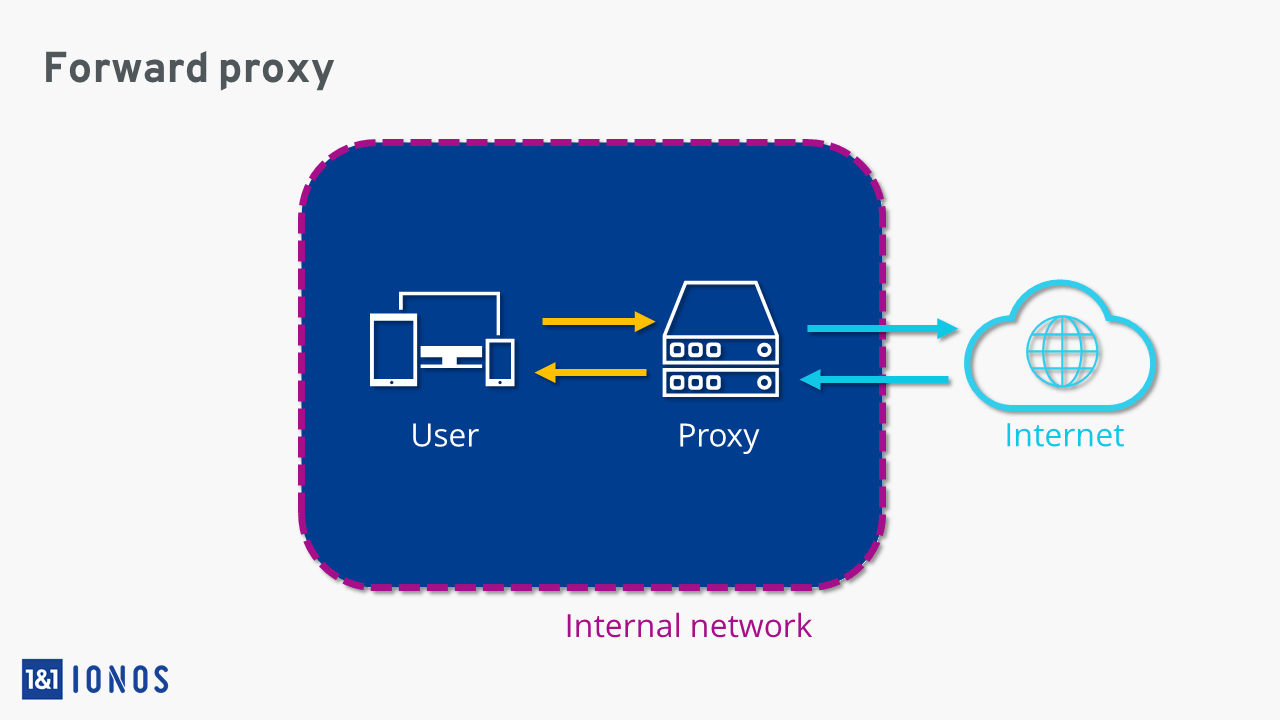
\includegraphics[width=0.45\textwidth]{images/proxy}
	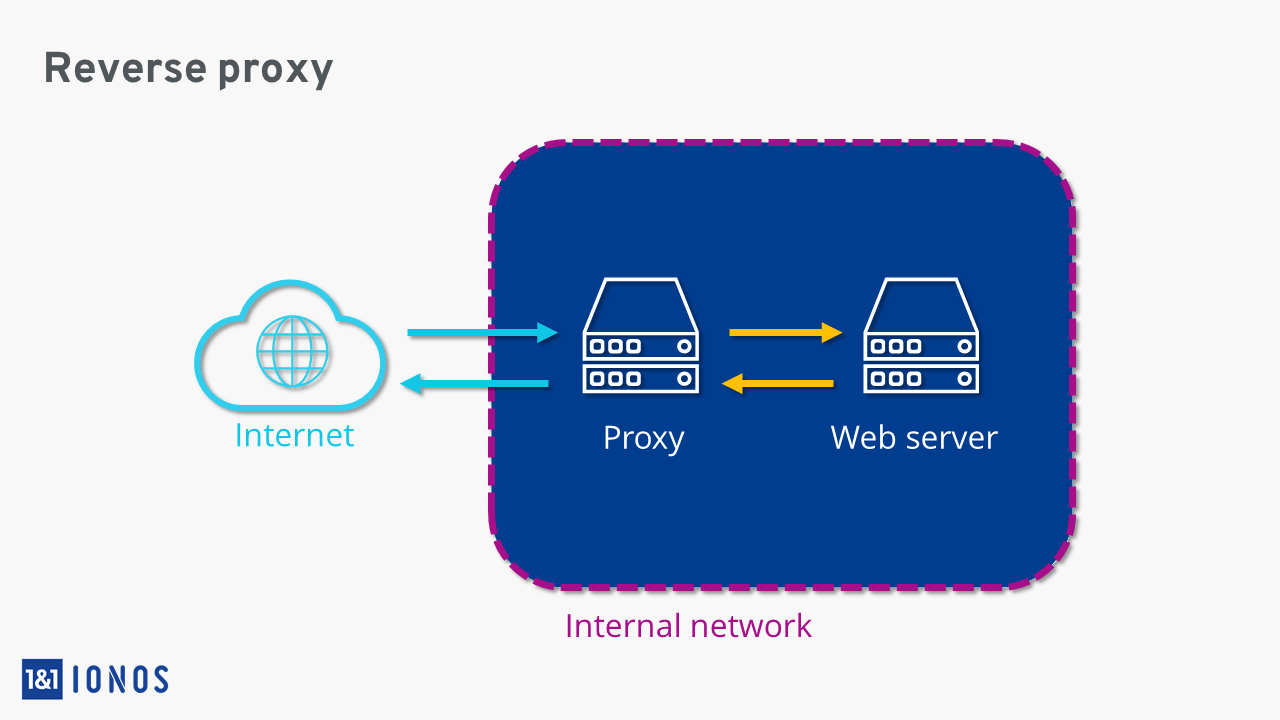
\includegraphics[width=0.45\textwidth]{images/proxyInverso}
	\caption{Esquema de un \emph{proxy} frente a un \emph{proxy} inverso. Imágenes de \url{https://www.ionos.es/digitalguide/servidores/know-how/que-es-un-servidor-proxy-inverso}.}
\end{figure}

Como se puede inferir de las definiciones anteriores, el uso de un \emph{proxy} inverso no queda restringido a ciertas arquitecturas, pudiéndose utilizar para ocultar el servicio o servicios que consume cualquier aplicación. Sin embargo, este componente adquiere una gran importancia en el enfoque de microservicios, pues es importante no exponer estos al exterior. Además, se suele utilizar también para realizar tareas de balanceo de carga. La figura \ref{figura:proxyInverso_o_no} muestra la comparativa de una arquitectura de microservicios básica y otra que utiliza el componente comentado. En la segunda se observa que con el uso de un \emph{proxy} inverso los clientes no acceden directamente a los microservicios, ni siquiera los conocen.

\begin{figure}[ht]
	\centering
	\label{figura:proxyInverso_o_no}
	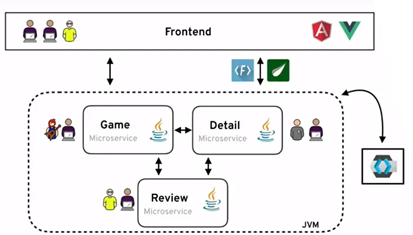
\includegraphics[width=0.45\textwidth]{images/arquitecturaMicroserviciosBasica}
	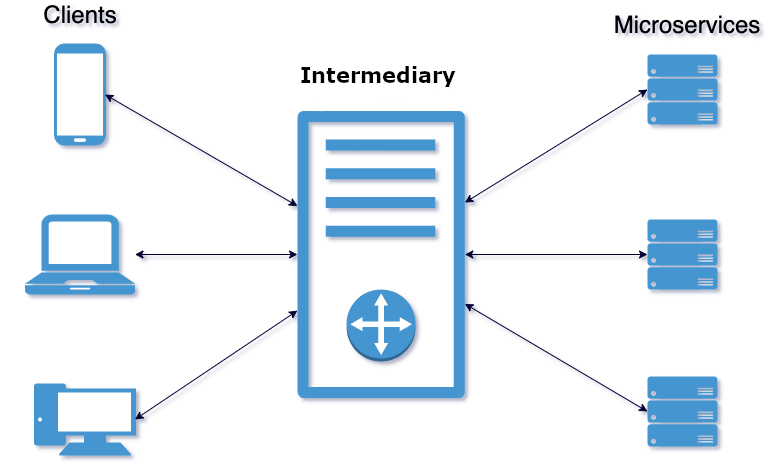
\includegraphics[width=0.45\textwidth]{images/arquitecturaMicroserviciosConProxyInverso}
	\caption{Arquitectura de microservicios básica frente a una con \emph{proxy} inverso. Imágenes de \url{https://www.adictosaltrabajo.com/2020/05/27/introduccion-al-api-gateway-pattern}.}
\end{figure}

\section{Motivación}

Este proyecto surge en el contexto de una práctica en empresa. El autor del mismo ha formado parte del equipo de \emph{I+D+i} de una compañía española del sector sociosanitario. Esta desarrolla y comercializa un \emph{software} de gestión geriátrica y actualmente se encuentra en periodo de renovación del mismo. El departamento recién nombrado se dedica a reconstruirlo desde cero con tecnología de vanguardia como el uso de arquitecturas de microservicios, el desarrollo de software dirigido por modelos y la generación automática de código.

La temática del trabajo es el desarrollo de un \emph{proxy} inverso que actúe de intermediario entre la interfaz de usuario de la nueva aplicación en desarrollo y sus microservicios. Se pretende construir este nuevo componente porque se cree necesario proteger el \emph{backend} de la aplicación y ocultar los microservicios que lo forman. Por otro lado, también se quiere tener la posibilidad de lanzar a ejecución múltiples instancias de los microservicios con el fin de conseguir cierta tolerancia a fallos y poder también realizar balanceo de carga.

La temática comentada fue elegida debido a la estrecha relación que guarda con el desempeño del autor en las prácticas mencionadas, esto es, contribuciones a un microservicio específico destinado a orquestar el despliegue de la aplicación. Por otro lado, el desarrollo a llevar a cabo le va a otorgar una visión más global de la aplicación sobre la que se trabaja así como aumentar el nivel de conocimiento acerca de la misma con la motivación de seguir contribuyendo al proyecto por mucho tiempo más. Por último, la tecnología a utilizar, \emph{.NET}, es de su interés y aspira así a crecer como desarrollador de ese \emph{framework}. En cuanto a la motivación de la empresa, esta quiere dar la posibilidad de aprovechar, en cierta medida, el trabajo realizado y a realizar por el autor del documento dentro del marco de trabajo de la entidad, viéndose esta beneficiada también.

\section{Objetivos}

El objetivo principal de este trabajo es construir un \emph{proxy} inverso. La construcción de este tiene las siguientes aspiraciones sobre la aplicación en construcción:

\begin{itemize}

	\item \textbf{Ocultar los microservicios} que forman la aplicación para que la interfaz de usuario no acceda directamente a estos por motivos de seguridad.
	
	\item Permitir la \textbf{instanciación múltiple} de los microservicios que, a su vez, tiene por finalidad:
		\begin{itemize}
		
			\item Conseguir que la aplicación sea \textbf{tolerante a fallos}, gracias a la posibilidad de tener un mismo microservicio desplegado en máquinas diferentes.
			
			\item \textbf{Aumentar la eficiencia}, al poder crear o parar instancias dinámicamente según el tráfico que reciba la aplicación.
			
		\end{itemize}

\end{itemize}

\section{Estructura del documento}

?????

%%%%%%%%%%%%%%%%%%%%%%%%%%%%%% ESTADO DEL ARTE %%%%%%%%%%%%%%%%%%%%%%%%%%%%%%

\chapter{Estado del arte}

comrpar y usar (estado del arte) vs libreria base
En la actualidad existen en el mercado muchas aplicaciones y servicios que resuelven problemas parecidos al planteado. Estas herramientas se pueden dividir en dos tipos: los \emph{API Gateway} y los \emph{proxy} inversos. Ambos patrones comparten algunos casos de uso, por lo que sus diferencias causan confusión y no suelen quedar claras. Generalmente, se entiende que un \emph{API Gateway} es una especialización de un \emph{proxy} inverso, proporcionando así funcionalidades extra. Las más aceptadas e importantes son:

\begin{itemize}

	\item Interpretan los mensajes que reciben y pueden hacer transformaciones sobre ellos; los \emph{proxy} inversos solo los redirigen donde corresponda.
	\item Suelen ofrecer agregaciones de peticiones, esto es, aunar dos o más llamadas al \emph{backend} y exponer esta composición a través de un único \emph{endpoint}.
	\item Realizan tareas transversales a todos los microservicios como autenticación, autorización o monitorización.

\end{itemize}

Algunos de estos productos \emph{software} son de pago, otros gratuitos e incluso algunos de código abierto. Se comentan los más relevantes a continuación.

\section{\emph{Kong}}
Tal y como dice su página web, \emph{Kong} \cite{Kong} es el \emph{API Gateway} más conocido a nivel mundial. Cuenta con las siguientes características:

\begin{itemize}

	\item Está optimizado para arquitecturas de microservicios.
	\item Está concebido para ser altamente escalable.
	\item Ha sido creado sobre el \emph{proxy} inverso \emph{NGINX}, lo que hace que su eficiencia destaque.
	\item Es gratuito, aunque ofrece la versión \emph{Enterprise}, que facilita la gestión del API Gateway, y la \emph{SaaS}, llamada \emph{Kong Cloud}.
	\item Posee un gran número de \emph{plugins} desarrollados por la propia compañía y por su comunidad, que es bastante grande al ser una aplicación tan popular.
	\item Actualmente es utilizado por grandes empresas como \emph{Intel}, \emph{Ferrari} o \emph{Yahoo!}.

\end{itemize}

\section{\emph{Tyk}}
\emph{Tyk} \cite{Tyk} es un \emph{API Gateway} de código abierto.

\begin{itemize}

	\item Permite alojar sus servicios tanto en la nube como en una infraestructura propia. También ofrece un modelo híbrido.
	\item Dispone de extensiones para integrarlo con diferentes mecanismos de autenticación como \emph{OAuth} o \emph{LDPA}.
	\item Necesita una base de datos \emph{Redis}.
	\item Puede escalar horizontalmente y verticalmente.

\end{itemize}

\section{\emph{Ocelot}}
\emph{Ocelot} \cite{Ocelot} es una librería para \emph{.NET Core} que permite a una aplicación de ese \emph{framework} actuar como API Gateway. Posee las características siguientes:

\begin{itemize}

	\item Está pensada para arquitecturas orientadas a servicios o a microservicios.
	\item Al tratarse de una librería, se utiliza de forma sencilla añadiéndola como un paquete \emph{NuGet} más.
	\item Su configuración es muy básica, teniendo que especificarla en un fichero \emph{json}.
	\item No permite cambiar su configuración de manera dinámica.

\end{itemize}

\section{\emph{NGINX}}
Originariamente \emph{NGINX} \cite{NGINX} fue construido para ser un servidor web, como por ejemplo \emph{Apache}, pero más tarde ofreció la posibilidad de actuar como \emph{proxy} inverso, balanceador de carga o \emph{proxy} para protocolos de correo electrónico. Desde la vertiente que interesa a este trabajo:

\begin{itemize}

	\item Se trata de un \emph{proxy} inverso ligero y de alto rendimiento
	\item Ofrece una versión gratuita y otra de pago, \emph{NGINX Plus}, la cual ofrece funcionalidades extra.
	\item Se configura a través de un fichero el cual puede ser recargado durante su ejecución, es decir, es configurable dinámicamente.

\end{itemize}

\section{Comparativa}

?????

\section{Tecnología utilizada}

La tecnología a utilizar para llevar a cabo este proyecto va a ser \emph{YARP} \cite{YARP}. Se trata de una librería hecha por el propio \emph{Microsoft}. Su objetivo es facilitar la creación de \emph{proxies} inversos. Sus aspectos más destacados son:

\begin{itemize}

	\item Se encuentra todavía en desarrollo y la única versión lanzada hasta la fecha es una \emph{preview}. Se prevé que vayan saliendo a la luz más versiones con más funcionalidades basadas en la experiencia de la propia empresa pero también en las opiniones de la gente.
	\item Fue diseñada para construir \emph{proxies} inversos dentro de la propia infraestructura de \emph{Microsoft} ya que en muchas áreas de la compañía necesitaban algo así.
	\item A raíz de la heterogeneidad de casos de uso que debe cubrir derivado del punto anterior, está pensada para ser muy personalizable y flexible.
	\item Permite cambiar su configuración de forma dinámica.

\end{itemize}

\subsection{Ejemplo de uso básico}

?????

%%%%%%%%%%%%%%%%%%%%%%%%%%%%%% DESARROLLO DE LA SOLUCIÓN %%%%%%%%%%%%%%%%%%%%%%%%%%%%%%

\chapter{Desarrollo de la solución}

?????

%%%%%%%%%%%%%%%%%%%%%%%%%%%%%% ESPECIFICACIÓN DE REQUISITOS %%%%%%%%%%%%%%%%%%%%%%%%%%%%%%

\section{Especificación de requisitos}

\begin{itemize}

	\item Redirección de peticiones
	\item Carga dinámica de rutas
	\item Eliminación de rutas
	\item Multi-instacia de microservicios
	\item Versionado de microservicios

\end{itemize}

\subsection{Diagrama de casos de uso}

?????

\subsection{Pruebas de aceptación}

?????

%%%%%%%%%%%%%%%%%%%%%%%%%%%%%% DISEÑO %%%%%%%%%%%%%%%%%%%%%%%%%%%%%%

\section{Diseño}

?????

\subsection{Diagrama de componentes}

?????

\subsection{Diagrama de clases}

?????

%%%%%%%%%%%%%%%%%%%%%%%%%%%%%% PROGRAMACIÓN %%%%%%%%%%%%%%%%%%%%%%%%%%%%%%

\section{Programación}

Para la construcción del \emph{proxy} inverso que protagoniza este trabajo se ha seguido una serie de pasos que se van a comentar a continuación.

\subsection{Construcción de prototipos}

El desarrollo comenzó con la elaboración de dos prototipos de microservicio con la funcionalidad mínima para redirigir peticiones. Estos prototipos tenían la misión de demostrar si era posible seguir la estructura general de todos los microservicios de la aplicación, con gran parte del código generado a partir de modelos. Precisamente este código autogenerado es lo que generaba ciertas dudas con lo referente al rendimiento final, el cual se podía ver perjudicado debido a un código menos específico y más genérico, así como a un exceso de características innecesarias para el caso en cuestión pero que sí debían poseer el resto de microservicios.

El primero de los prototipos se hizo lo más simple posible, es decir, con la lógica justa y necesaria para desempeñar su trabajo y sin seguir ninguna estructura concreta. El segundo, fue construido utilizando las mismas herramientas con las que fueron construidos el resto de microservicios de la aplicación, esto es, generación de código a partir de modelos. Cabe destacar que, para no realizar esfuerzos en vano sin saber qué prototipo iba a ser la opción elegida, se dejaron algunos detalles correspondientes a la generación de código pendientes. Esto se debe a que el proceso de generación de código no se adaptaba al cien por cien a las necesidades del nuevo microservicio.

Una vez construidos los prototipos, se procedió a medir el impacto de seguir la norma para decidir qué prototipo desechar y con cuál seguir adelante.

Los resultados de las mediciones fueron claros: ambos prototipos tenían un rendimiento casi idéntico. De esta forma, se decidió continuar con la versión autogenerada.

\subsection{Consolidación del microservicio autogenerado}

Una vez elegida la opción de seguir el estándar, hubo que resolver los aspectos de la generación de código que no quedaron resueltos. Así pues, se tuvo que modificar algunas plantillas de código a partir de las cuales se generan los microservicios. Por otro lado, también fue necesario abordar otros problemas derivados de seguir el patrón de microservicio estándar.

\subsection{Primeros despliegues}

A estas alturas del desarrollo ya se tenía una primera versión del \emph{proxy} inverso perfectamente funcional pero antes de llevar a cabo los primeros despliegues había que adaptarlo al proceso de despliegue que se seguía hasta el momento. La interfaz de usuario de la aplicación se conectaba directamente a los microservicios por lo que hizo falta interponer el nuevo componente entre ella y el \emph{backend}.

Más tarde, se hizo que los propios microservicios utilizaran el \emph{proxy} inverso para comunicarse entre ellos.

El único microservicio que no se pudo reemplazar fue el de autorización porque tenía una dirección específica, configurada a través del DNS.

Como paso previo a incluir el \emph{proxy} inverso al proceso de despliegue primero se hicieron pruebas de manera local. Se desplegó el \emph{proxy} inverso en una máquina a parte y se le cargó con rutas que apuntaban a los microservicios ya desplegados para que la interfaz de usuario lo utilizara. Se comprobó que todo funcionaba correctamente.

%%%%%%%%%%%%%%%%%%%%%%%%%%%%%% PRUEBAS %%%%%%%%%%%%%%%%%%%%%%%%%%%%%%

\section{Pruebas}

Durante el proceso de programación ya se realizaron pruebas.

%%%%%%%%%%%%%%%%%%%%%%%%%%%%%% CONCLUSIONES %%%%%%%%%%%%%%%%%%%%%%%%%%%%%%

\chapter{Conclusiones}

?????

%%%%%%%%%%%%%%%%%%%%%%%%%%%%%% BIBLIOGRAFÍA %%%%%%%%%%%%%%%%%%%%%%%%%%%%%%

\begin{thebibliography}{10}

\bibitem{LewisAndFowler}
	Artíclo de J. Lewis y M. Fowler acerca de los microservicios.
	\newblock Disponible en:\\
	\url{https://martinfowler.com/articles/microservices.html}

\bibitem{Newman}
	Libro de referencia sobre microservicios
	\newblock Sam Newman
	\newblock Building Microservices

\bibitem{Kong}
	Documentación oficial de \emph{Kong}:\\
	\url{https://konghq.com/kong}

\bibitem{Tyk}
	Documentación oficial de \emph{Tyk}:\\
	\url{https://tyk.io}

\bibitem{Ocelot}
	Documentación oficial de \emph{Ocelot}:\\
	\url{https://threemammals.com/ocelot}

\bibitem{NGINX}
	Documentación oficial de \emph{NGINX}:\\
	\url{https://www.nginx.com/}

\bibitem{YARP}
	Documentación oficial de \emph{YARP}:\\
	\url{https://microsoft.github.io/reverse-proxy}

\end{thebibliography}

\end{document}
